\documentclass{article}
% Chinese
% \documentclass[UTF8, nofonts, mathptmx, 12pt, onecolumn]{article}
% \usepackage{xeCJK}
% \setCJKmainfont{SimSun}
\usepackage{amsmath}
\usepackage{amsfonts}
\usepackage{amssymb}
\usepackage{wasysym}
% \usepackage{ctex}
\usepackage{graphicx}
\usepackage{float}
\usepackage{geometry}
\geometry{a4paper,scale=0.8}
\usepackage{caption}
\usepackage{subcaption}
% \newcommand{\oiint}{\mathop{{\int\!\!\!\!\!\int}\mkern-21mu \bigcirc} {}}
\newcommand*{\dif}{\mathop{}\!\mathrm{d}}
\newcommand*{\md}{\mathop{}\!\mathrm{d}}
\newcommand*{\me}{\mathrm{e}}

\usepackage{parskip}
\setlength{\parindent}{0cm}

\usepackage{bm}
\let\Oldmathbf\mathbf
\renewcommand{\mathbf}[1]{\boldsymbol{\Oldmathbf{#1}}}
\let\eqnarray\align

\author{Xiping Hu}
\usepackage{authblk}
\author{Xiping Hu}
\affil{http://thehxp.tech/}
\title{Homework for Analogue Electronics}

\begin{document}
\maketitle

\begin{figure}[H]
  \centering
  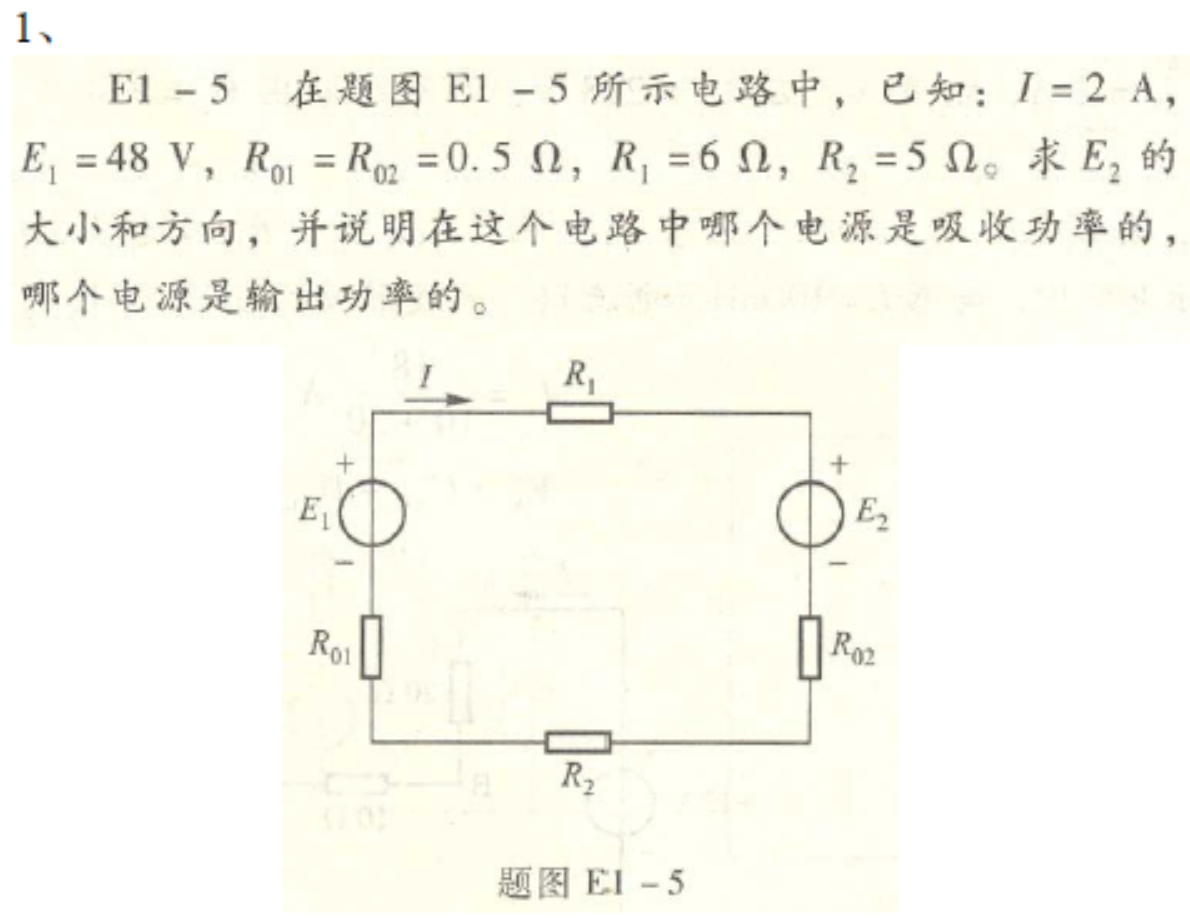
\includegraphics[width=\linewidth]{figures/1}
  \label{fig:}
\end{figure}

\paragraph{Solution}

According to KVL:

\begin{equation*}
  \begin{aligned}
    - I R_1 - E_2 - I R_{02} - I R_2 - I R_{01} + E_1 = 0 \\   
  \end{aligned}
\end{equation*}
\begin{equation*}
  \begin{aligned}
    - I R_1 - I R_{02} - I R_2 - I R_{01} + E_1 = E_2\\
    E_2 = - 12 - 1 - 10 - 1 + 48 = 24 \  \mathrm{V}
  \end{aligned}
\end{equation*}

From the current direction, which is clock-wised, we can know that $E_1$ is providing power, $E_2$ is consuming power.


\end{document}